\documentclass[11pt,compress,t,notes=noshow, aspectratio=169, xcolor=table]{beamer}

\usepackage{../../style/lmu-lecture}
% Defines macros and environments
% This file is included in slides and exercises

% Rarely used fontstyle for R packages, used only in 
% - forests/slides-forests-benchmark.tex
% - exercises/single-exercises/methods_l_1.Rnw
% - slides/cart/attic/slides_extra_trees.Rnw
\newcommand{\pkg}[1]{{\fontseries{b}\selectfont #1}}

% Spacing helpers, used often (mostly in exercises for \dlz)
\newcommand{\lz}{\vspace{0.5cm}} % vertical space (used often in slides)
\newcommand{\dlz}{\vspace{1cm}}  % double vertical space (used often in exercises, never in slides)
\newcommand{\oneliner}[1] % Oneliner for important statements, used e.g. in iml, algods
{\begin{block}{}\begin{center}\begin{Large}#1\end{Large}\end{center}\end{block}}

% Don't know if this is used or needed, remove?
% textcolor that works in mathmode
% https://tex.stackexchange.com/a/261480
% Used e.g. in forests/slides-forests-bagging.tex
% [...] \textcolor{blue}{\tfrac{1}{M}\sum^M_{m} [...]
% \makeatletter
% \renewcommand*{\@textcolor}[3]{%
%   \protect\leavevmode
%   \begingroup
%     \color#1{#2}#3%
%   \endgroup
% }
% \makeatother


\title{Interpretable Machine Learning}
% \author{LMU}
%\institute{\href{https://compstat-lmu.github.io/lecture_iml/}{compstat-lmu.github.io/lecture\_iml}}
\date{}

\bibliography{feature-importance}

%\usepackage{Sweave}
\begin{document}
	\newcommand{\titlefigure}{figure_man/feature-importance.png}
    \newcommand{\learninggoals}{
    	\item Definition of LOCO
    	\item Interpretation of LOCO}
	% Set style/preamble.Rnw as parent.
	
	% Load all R packages and set up knitr
	
	% This file loads R packages, configures knitr options and sets preamble.Rnw as 
	% parent file
	% IF YOU MODIFY THIS, PLZ ALSO MODIFY setup.Rmd ACCORDINGLY...
	
	% Defines macros and environments

	\lecturechapter{Leave One Covariate Out (LOCO)}
	\lecture{Interpretable Machine Learning}
	
	% ------------------------------------------------------------------------------

\begin{vbframe}{Reminder: Feature Importance Scheme}
In general, feature importance methods share two components
\lz
\begin{enumerate}
  \item \textbf{Perturbation/Removal:} Generate predictions for which the feature of interest has been perturbed/removed.
  \item \textbf{Performance Comparision:} Compare performance under perturbation/removal with the original model performance.
\end{enumerate}
\lz
Depending on the type of perturbation/removal feature importance methods provide insight into different aspects of model and data.\\
\lz
\textbf{LOCO idea:} Simply remove the feature from the dataset and refit the model on the reduced dataset. The performance loss compared to the full model is interpreted as feature importance.\\

\end{vbframe}

\begin{vbframe}{Leave One Covariate Out (LOCO)}
% citation of the original LOCO paper
%
\textbf{Definition:} Given training and test datasets $\Dtrain, \Dtest \subseteq \D$, some $\inducer$ and a model $\fh = \inducer(\Dtrain)$. Then LOCO for a feature $j \in \pset$ can be computed as follows:
  \begin{enumerate}
    \item learn model on dataset ${\Dtrain}_{,-j}$ where feature $x_j$ was removed, i.e. $\fh_{-j} = \inducer({\Dtrain}_{,-j})$
    \item compute the difference in local $L_1$ loss for each element in $\Dtest$, i.e. $\Delta_j^{(i)} = \left  |y^{(i)} - \fh_{-j}(x_{-j}^{(i)}) \right | - \left |y^{(i)} - \fh(x^{(i)}) \right | $ with $i \in \Dtest$
    \item yield the importance score $\text{LOCO}_j = \text{med} \left ( \Delta_j  \right )$
  \end{enumerate}
\lz 
The method can be generalized to other loss functions and aggregations. If we use mean instead of median we can rewrite LOCO as
%
$$ \text{LOCO}_j = \riske(\fh_{-j}) - \riske(\fh).$$
\footnote[frame]{\fullcite{lei_distribution-free_2018}\\ \fullcite{tibshirani_loco_2018}}
\end{vbframe}

\begin{vbframe}{Bike Sharing Example}
%
\begin{figure}
  \centering
  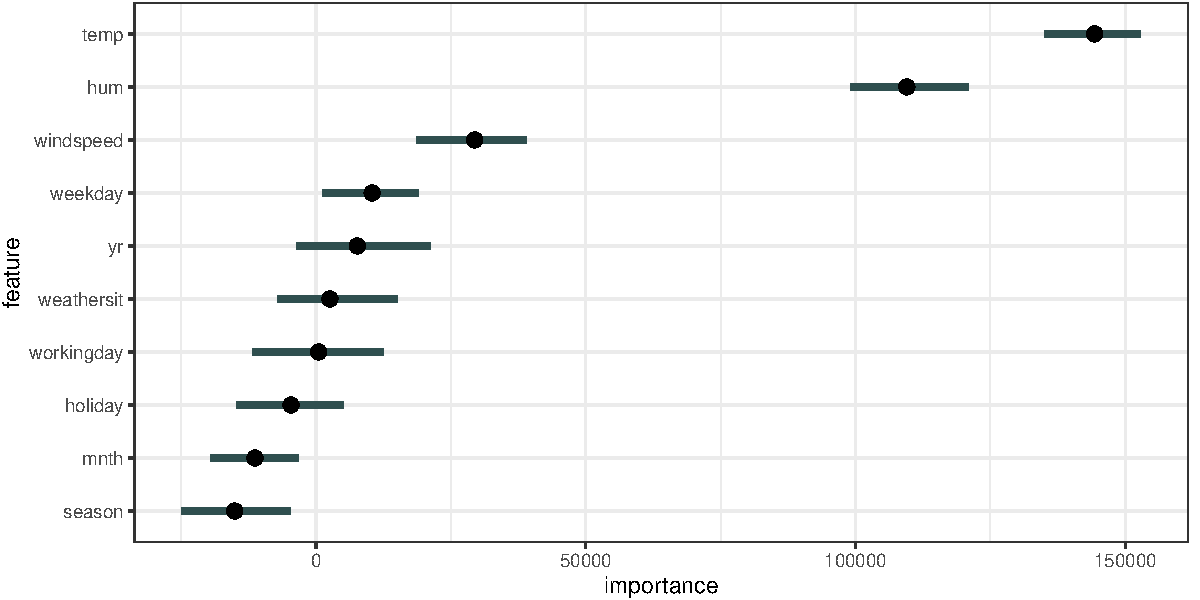
\includegraphics[width=0.65\textwidth]{figure_man/bike_sharing_loco.pdf}
\caption{A random forest with default hyperparameters was fit on $70\%$ of the bike sharing dataset to optimize MSE. Then LOCO was computed for all features on the training dataset. The year is the most important feature. Without access to the variable, the MSE increases by $10^6$.}
\end{figure}
%
 %\textbf{Interpretation:} $\text{LOCO}_j$ quantifies how important variable $x_j$ is to the generalization performance of the learner on $\Dtrain$.\\
%
\end{vbframe}

\begin{vbframe}{Interpretation of LOCO}

\textbf{Interpretation:} LOCO estimates the generalization error of the learner on a reduced dataset $\D_{-j}$.\\
\lz
Can we get insight into whether ...
\begin{enumerate}
    \item the feature $x_j$ is causal for the prediction $\yh$?
    \begin{itemize}
      \item In general, no (counterexample on the next slide).
    \end{itemize}
    \item the variable $x_j$ contains prediction-relevant information?
    \begin{itemize}
      \item In general, no (counterexample on the next slide).
    \end{itemize}
    \item the model requires access to $x_j$ to achieve it's prediction performance?
    \begin{itemize}
      \item Approximately. It provides insight into whether the \textit{learner} requires access to $x_j$.
    \end{itemize}
\end{enumerate}
\end{vbframe}

\begin{vbframe}{Interpretation of LOCO}

\begin{figure}
\centering
%\hfill
 % \begin{tikzpicture}[thick, scale=1.1, every node/.style={scale=0.6, line width=0.3mm, black, fill=white}]
%		\node[draw, circle, font=\large] (x1) at  (-.5, 2) {$X_1$};
%		\node[draw, circle, font=\large] (x2) at  (-.5,1) {$X_2$};
%		\node[draw, circle, font=\large] (x3) at  (.5,1) {$X_3$};
%		\node[draw, circle, font=\large] (y) at  (0,0) {$Y$};
%		\draw[->, black] (x1) -- (x2);
%		\draw[->, black] (x3) -- (y);
%		\draw[->, black] (x2) -- (y);
%	\end{tikzpicture} 
\hfill
	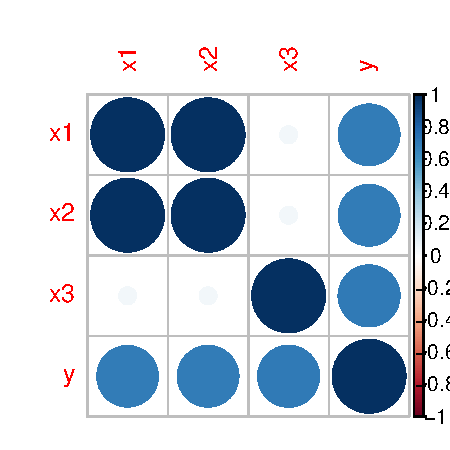
\includegraphics[width=0.25\linewidth]{figure_man/simulation_corr.pdf} 
\hfill
  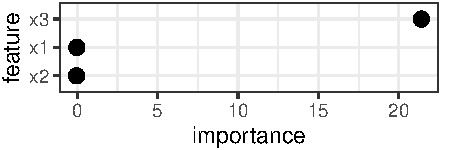
\includegraphics[width=0.5\linewidth]{figure_man/simulation_loco}
  \hfill
\end{figure}

Setting: Linear gaussian data generating process with correlation matrix as depicted left. A linear model was fit with $\fh(x) = -0.09 - 0.86 x_1 + 1.86 x_2 + 0.96 x_3$.\\
\lz
$\Rightarrow$ At the example of $x_2$ we see that: We cannot infer (1) from LOCO (e.g. $\text{LOCO}_2 \approx 0$ but coefficient $1.86$) (1). We also can't infer (2), e.g. $corr(x_2, y) = 0.69$ but $\text{LOCO}_2 \approx 0$.\\
$\Rightarrow$ We can get insight into (3). Since $x_2$ and $x_1$ are highly correlated, they can take each others place, which is not the case for $x_3$.
\framebreak


\end{vbframe}

\begin{vbframe}{Pros and Cons}
  Pros:
  \begin{itemize}
    \item Requires (only?) one resampling set per feature for evaluation
    \item Easy to implement
    \item Testing framework available in \cite{lei_distribution-free_2018}
  \end{itemize}
%
  Cons:
  \begin{itemize}
    \item Does not provide insight into a specific model, but rather a learner on a specific dataset.
    \item Model training is a random process, so estimates can be noisy (which is problematic for inference about model and data).
  \end{itemize}
\end{vbframe}

\begin{vbframe}{Bibliography}
  \printbibliography
\end{vbframe}

\endlecture
\end{document}
